%% Adaptado a partir de :
%%    abtex2-modelo-trabalho-academico.tex, v-1.9.2 laurocesar
%% para ser um modelo para os trabalhos no IFSP-SPO

\documentclass[
    % -- opções da classe memoir --
    12pt,               % tamanho da fonte
    openright,          % capítulos começam em pág ímpar (insere página vazia caso preciso)
    %twoside,            % para impressão em verso e anverso. Oposto a oneside
    oneside,
    a4paper,            % tamanho do papel. 
    % -- opções da classe abntex2 --
    %chapter=TITLE,     % títulos de capítulos convertidos em letras maiúsculas
    %section=TITLE,     % títulos de seções convertidos em letras maiúsculas
    %subsection=TITLE,  % títulos de subseções convertidos em letras maiúsculas
    %subsubsection=TITLE,% títulos de subsubseções convertidos em letras maiúsculas
    % Opções que não devem ser utilizadas na versão final do documento
    %draft,              % para compilar mais rápido, remover na versão final
    MODELO,             % indica que é um documento modelo então precisa dos geradores de texto
    %TODO,               % indica que deve apresentar lista de pendencias 
    % -- opções do pacote babel --
    english,            % idioma adicional para hifenização
    brazil              % o último idioma é o principal do documento
   ]{ifsp-spo-inf-ctds}
\graphicspath{ {./images/} }
% ---

% --- 
% CONFIGURAÇÕES DE PACOTES
% --- 
%\usepackage{etoolbox}
%\patchcmd{\thebibliography}{\chapter*}{\section*}{}{}


% ---
% Informações de dados para CAPA e FOLHA DE ROSTO
% ---
\titulo{Metaverso - Ferramenta de Chamados de TI (ITSM) para pessoas físicas e pequenas empresas}

% Trabalho individual
%\autor{JOSÉ BRAZ DE ARAUJO}

% Trabalho em Equipe
% ver também https://github.com/abntex/abntex2/wiki/FAQ#como-adicionar-mais-de-um-autor-ao-meu-projeto
\renewcommand{\imprimirautor}{
\begin{tabular}{lr}
%CEZAR GODOY NASCIMENTO	& SP3040755 \\
HENRIQUE HIROMI SHIMADA & SP3039421 \\
ISABELA SOUZA DUARTE	& SP3030083 \\
MATEUS SOUZA DA SILVA	& SP3022374 \\
VINICIUS GOMES MOREIRA	& SP3039587 \\
WELEN MOTA SOUSA	& SP146616X \\
\end{tabular}
}


\tipotrabalho{Projeto da Disciplina Projeto Integrado I}

\disciplina{PI1A5 - Projeto Integrado I}

\preambulo{Proposta de projeto para disciplina PI1A5}

\data{MARÇO DE 2022}

% Definir o que for necessários e comentar o que não for necessário
% Utilizar o Nome Completo, abntex tem orientador e coorientador
% então vão ser utilizados na definição de professor
\renewcommand{\orientadorname}{Professor:}
\orientador{JOSE BRAZ DE ARAUJO}
\renewcommand{\coorientadorname}{Professor:}
\coorientador{MARCELO TAVARES DE SANTANA}



% ---


% ---
% Configurações de aparência do PDF final


% informações do PDF
\makeatletter
\hypersetup{
        %pagebackref=true,
        pdftitle={\@title}, 
        pdfauthor={\@author},
        pdfsubject={\imprimirpreambulo},
        pdfcreator={LaTeX with abnTeX2},
        pdfkeywords={abnt}{latex}{abntex}{abntex2}{trabalho acadêmico}, 
        colorlinks=true,            % false: boxed links; true: colored links
        linkcolor=blue,             % color of internal links
        citecolor=blue,             % color of links to bibliography
        filecolor=magenta,              % color of file links
        urlcolor=blue,
        bookmarksdepth=4
}
\makeatother
% --- 

% ---

% ----
% Início do documento
% ----
\begin{document}

% Retira espaço extra obsoleto entre as frases.
\frenchspacing 

\pretextual

% ---
% Capa - Para proposta a folha de rosto é suficiente pois é mais completa.
% ---
\imprimirfolhaderosto
% ---

% ----------------------------------------------------------
% ELEMENTOS TEXTUAIS
% ----------------------------------------------------------
\textual

\chapter[Introdução]{Introdução}

	De acordo com a PNAD de 2019 (\citeauthor{PNAD:2019}), 82,7\% dos domicílios brasileiros contam com acesso à internet. Mesmo tendo acesso de banda larga em 80,2\% dos dispositivos móveis do país, apenas 45,1\% os domicílios da amostra têm acesso via computador. Assim, entendemos que embora muitos dos usuários têm alguma fluência em aplicativos móveis, as diferenças de interfaces pode ser um desafio para o usuário que têm tarefas diferentes das desempenhadas em aplicativos móveis.

	Ainda, considerando que existem diversas soluções corporativas de suporte, em contraste, para esses usuários, as soluções que mais se apresentam são fóruns, que ainda que sejam gratuitas, ainda demandam algum trabalho e interação que os usuários alvo são pouco familiarizados ou têm compreensão limitados em relação à dinâmica de tais ferramentas.

	Assim, propomos uma ferramenta com capacidade de suportar os usuários que sentem necessidade de suporte personalizado.

\chapter[Problema]{Problema}

% Dificuldade em resolver problemas corriqueiros incomodam ou impedem o uso esperado do dispositivo, como um mal funcionamento de impressora e lentidão na execução de softwares, tornando sua utilização menos produtiva.

Existência de potencial relevante de usuários de pouca fluência com soluções de tecnologia que têm dificuldades em resolver problemas frustantes e corriqueiros com computadores pessoais que  incomodam ou impedem o uso esperado do dispositivo por não conseguirem desfrutar do dispositivo ou, mesmo, trabalhar.

\begin{comment}
\subsection{Personas}
Usuários finaliza com nível muito elementar de conhecimento e interação com dispositivos desktop.

\subsubsubsection{Persona 1}
José é um senhor de 65 anos que sempre trabalhou em escritórios, mas sempre contou com o suporte da empresa em que trabalhava para conseguir resolver problemas cotidianos. Entretanto, desde que se aposentou, não conta mais com esse suporte. Não é um problema muito grande, mas nem sempre existe alguém disponível para ajuda-lo e o problema acaba esquecido. Seu computador novo só é usado, quando está no cabo.

\subsubsubsection{Persona 2}
Eleonora é uma enfermeira que usa apenas os sistemas do hospital em que trabalha. Em casa, preciso instalar o sistema java no seu computador para fazer a declaração do imposto de renda do ano em seu computador novo, mas morre de fazer algo e ter dados vazados. Não sabe pra quem pedir, por que está sempre muito ocupada.

\subsubsubsection{Persona 3}
Rafael é pai de duas crianças pequenas e trabalha o dia inteiro na rua, mas precisa emitir nota fiscal e fazer algumas coisas no computador de tempos em tempos. Entretanto vira e mexe, tem que resolver problemas com o computador ou com a impressora e isso sempre toma tempo demais, tomando do tempo que gostaria de brincar com os filhos.

\subsubsubsection{Persona 4}
Claudenice faz a melhor coxinha da região e é muito organizada. Os negócios estão indo muito bem e até já contratou uma contabilidade e duas pessoas para ajudar a organizar nas atividades do dia a dia. Mas, nenhuma das pessoas que contratou pode fazer algo que ela não abre mão: tomar conta das próprias finanças. Mesmo assim, vão ajuda-la a organizar as entregas e coletar os pedidos no computador. Ninguém sabe mexer muito bem no computador e isso preocupa a Claudenice, pois já ficou na mão uma vez e demorou bastante para conseguir achar alguém que ajudasse.



\chapter{Modelo de negócio}

O modelo de negócio contará com planos free e escalonado em dois diferentes níveis de serviço para permitir que os clientes possam escolher o nível de suporte que deseja ser atendido.

Em ambos os modos, existe a possibilidade do usuário, após passar pelos filtros da plataforma para sua solução de problema, acionar um prestador de serviços terceiro, que poderá atender o usuário presencialmente em seu estabelecimento. Nesses casos, a plataforma poderá receber o pagamento do serviço (tabelado) e reter o mesmo até confirmação da solução por ambas as partes, funcionando como uma intermediadora.


Futuramente, poderão ser estudados planos de assinaturas premium em níveis diferenciados.

\section{Planos}

\subsection{Free}

Usuário acessa a plataforma, navega pelos FAQs, podendo sanar suas dúvidas e resolver seus problemas por conta própria através da plataforma – Contém ADS.

\subsection{Premium}

Modelo de assinatura mensal onde o usuário paga um valor e terá 1 dispositivo vinculado à assinatura. Ao assinar, a equipe instalará os softwares para acesso remoto e, quando o usuário não conseguir resolver por conta própria o problema, será atendido via chat ou WhatsApp para resolução.


\section{MVP}

A proposta inicial é a criação de uma ferramenta que favoreça a identificação da solução pelo usuário por conta própria, utilizando orientação de uma solução automatizada.

Nesse momento, o desenvolvimento de uma solução que popule e atualize a seção de perguntas frequentes e o chat automatizado é prioridade de desenvolvimento e será o principal indicador de viabilidade.

\end{comment}


\chapter[Objetivos]{Objetivos}

	O projeto elaborado propõe uma solução que atenda pessoas com baixa fluência em sistemas de computação em situações cotidianas em que seus dispositivos não funcionem de acordo com o esperado pelo usuário.
	
	Entende-se que a solução tem como alvo pessoas físicas e pequenas empresas, que normalmente têm acesso limitado ou nenhum a ferramentas tradicionais de suporte de tecnologia da informação (\textit{ITSM - Information Technology Service Management}).
	
	Para tanto, foram definidos os seguintes objetivos para criação do serviço: elaboração do mínimo produto viável e suas ferramentas essenciais, com pontos de checagem (\textit{check point}) para verificação do avanço da solução.

\section{Objetivo Principal}

	Prover assistência a problemas em sistemas computacionais domésticos ou de pequenas empresas para usuários finais com pouca ou nenhuma familiaridade a problemas cotidianos.

\section{Objetivos Secundários}

	Para que o produto de ITSM - \textit{Information Technology Service Management} seja considerado viável, será necessário que as seguintes ferramentas sejam disponibilizadas as funcionalidades a seguir: 
	
	\begin{itemize}
		
		\item
		Familiarizar o usuário com pouca habilidade para resolver problemas de soluções simples com computadores pra que possam ser independentes;
		
		\item
		Facilitar a identificação e aplicação de resolução a problemas com computadores;
		
		\item
		Orientar os gestores da ferramenta sobre as questões e dificuldades mais comuns;
		
		\item 
		Facilitar o processo de resolução em caso de atendimento por terceiro credenciado
		 
	\end{itemize}

\chapter{Ferramentas}

\section{Ferramenta de respostas rápidas para perguntas frequentes: FAQ - \textit{Frequently Asked Questions}}

	Para a solução de FAQ, compreendeu-se a necessidade de desenvolvimento das ferramentas:
	
	\begin{enumerate}
		
		\item 
		Modelo de árvore de decisão
		
		Realização de consultar em banco de dados relacional baseado em SQL - \textit{Server Query Language}, o qual localiza uma resposta de solução ao problema alegado.
		
		\item 
		Tela inicial
		
		Implementação de ferramenta de busco para agregar na consulta otimizada afim de facilitar a procura de problemas relacionados.
		
		\item 
		Adicionar Cookie de sessão para armazenar o comportamento do usuário. (verificar IP - \textit{Internet Protocol} - público e contexto LGPD - Lei Geral de Proteção de Dados)
		
		Armazenamento do IP público do usuário para identificar o seu comportamento no site, seguindo critérios de aceite aos termos e políticas condicionais no site, baseadas na LGPD.
		
		\item 
		Cadastro no FAQ
		
		O cadastro no FAQ é realizado pelo próprio time da central de suporte técnico, quando identificam um novo problema que está sendo relatado com muita frequência, busca uma solução otimizada e disponibiliza no FAQ. 
		
	\end{enumerate}

\section{Login}

	\begin{enumerate}
		
		\item 
		Login confiável por autorização de acesso
		
	\end{enumerate}

\section{Cadastros}

	\begin{enumerate}
		
		\item 
		Criação de cadastro de perfil
		
		Após a realização do cadastro com o mínimo necessários de informação o cliente poderá fazer um preenchimento complementar do seu perfil, demonstrando:
		
			\begin{enumerate}
				
				\item 
				Marcas e modelos de seus equipamentos;
				
				\item
				Quantidade de usuários e nome dos usuários no local;
				
				\item
				Software de que gosta de utilizar;
				
				\item
				Outras opções.
				
			\end{enumerate}
		
		\item 
		Criação de cadastro de perfil técnico
		
		Após a realização do cadastro com o mínimo necessários de informação o cliente poderá fazer um preenchimento complementar do seu perfil, demonstrando
		
			\begin{enumerate}
				
				\item
				Marcas e modelos de seus equipamentos que atende;
				
				\item
				Formação profissional;
				
				\item
				Especialização;
				
				\item
				Área que realizará o atendimento de preferência;
				
				\item
				Outras opções. 
				
			\end{enumerate}
		
		\item
		Página de Cursos e Capacitação
		
		Os técnicos terão acesso a cursos que poderão realizar na plataforma afim de aprimorar o atendimento e capacitação e precisaram realizar uma avaliação técnica básica para realizar o atendimento.
		
	\end{enumerate}

\section{Visualização do perfil e escolha personalizada do técnico}

	\begin{enumerate}
		
		\item
		Visualização de cadastro de perfil
		
		O cliente poderá receber o perfil do técnico e sua média de avaliação e suas especialidades.
		
		\item
		Escolha de técnicos personalizada por critérios de avaliação
		
		O cliente poderá por meio de um plano especifico contratar um técnico com um perfil adequado a sua necessidade e baseado em sua avaliação.
		
	\end{enumerate}

\section{Agendamento de visita técnica}

	O cliente poderá por meio de um plano especifico contratar um técnico com um perfil adequado a sua necessidade e baseado em sua avaliação.

	\begin{enumerate}
	
	     \item
	     Ter opção de botão dedicado para o usuário final abrir um chamado de visita técnica on site.
	     
	     Opção de chamado técnico facilitado, o cliente com um cadastro simples, sem necessidade de acessar o FAQ poderá solicitar um técnico até o local, sendo guiado pelo processo de agendamento.
	     
	     \item
	     Agendamento por meio de raio de localidade
	     
	     Durante o processo de agendamento a escolha do técnico e feita é realizado por localidade do técnico registrado em uma determinada região.
	        
	\end{enumerate}

\section{Operacional}

	\begin{enumerate}
		
		\item
		Abertura do chamado técnico
		
		Todos os atendimentos técnicos realizados pela central de atendimento ou diretamente na visita técnica vão gerar uma abertura de um chamado técnico (incidente).
		
		\item
		Envio de foto do problema do equipamento
		
		O chamado possui campo para adicionar fotos do problema técnico alegado pelo cliente para armazenamento de histórico.
		
	\end{enumerate}

\section{Planos de Compra}

	\begin{enumerate}
		
		\item
		Free
		
		Usuário acessa a plataforma, navega pelos FAQs, podendo sanar suas dúvidas e resolver seus problemas por conta própria através da plataforma – Contém ADS.
		
		\item
		Basic
		
		Modelo de assinatura mensal onde o usuário paga um valor e terá 1 dispositivo vinculado à assinatura. Ao assinar, a equipe instalará os softwares para acesso remoto e, quando o usuário não conseguir resolver por conta própria o problema, será atendido via chat ou WhatsApp para resolução. Para atendimento técnico, os técnicos são escolhidos de forma aleatória dando preferência a região.
		
		\item
		Premium
		
		Modelo de assinatura mensal onde o usuário paga um valor e terá 5 dispositivos vinculado à assinatura. Ao assinar, a equipe instalará os softwares para acesso remoto e, quando o usuário não conseguir resolver por conta própria o problema, será atendido via chat ou WhatsApp. Para atendimento técnico, os técnicos são escolhidos de forma aleatória dando preferência a região e escolha de técnicos mais bem avaliados.
		
	\end{enumerate}

\section{Avaliação da visita técnica.}

	\begin{enumerate}
		
		\item
		Botão de Resolução (Sim ou Não)
		
		Após a conclusão da visita técnica aparecerá para o cliente uma pergunta se o problema foi resolvido com dois botões (Sim e Não), caso tenha resolvido apresentará a mensagem de dúvidas, sugestões ou reclamações. Em caso de não solução o incidente voltará a ser reportado para o time de atendimento técnico analisar o caso. 
		
		\item
		Avaliação da visita técnica
		
		Funcionalidade de avaliação da visita técnica do cliente com critérios de nota:(1 muito pouco satisfeito, 2 pouco satisfeito, 3 regular, 4 satisfeito, 5 muito satisfeito), o qual os técnicos mais bem avaliados terão mais chances de receber um contato de visita técnica. Existindo campos também para sugestões e reclamações.
		
	\end{enumerate}

\section{Modo de visualização}

	\begin{enumerate}
	
		\item
		Modo de aplicação em WEB
		
		O serviço será disponibilizado em formato de aplicação WEB acessível em qualquer navegador com interação facilitada.
		
		\item
		Avaliação da visita técnica.
		
		O serviço será disponibilizado em formato de aplicação WEB acessível em qualquer navegador com interação facilitada.
		
	\end{enumerate}

\section{Avaliação de visita técnica e clientes}

	\begin{enumerate}
		
		\item Avaliação da visita técnica.
		
		Funcionalidade de avaliação da visita técnica do cliente com critérios de nota:(1 muito pouco satisfeito, 2 pouco satisfeito, 3 regular, 4 satisfeito, 5 muito satisfeito), o qual os técnicos mais bem avaliados terão mais chances de receber um contato de visita técnica. Existindo campos também para sugestões e reclamações.
	
	
		\item Avaliação da visita técnica.
		
		Funcionalidade de avaliação da visita técnica do cliente com critérios de nota:(1 muito pouco satisfeito, 2 pouco satisfeito, 3 regular, 4 satisfeito, 5 muito satisfeito), o qual os técnicos mais bem avaliados terão mais chances de receber um contato de visita técnica. Existindo campos também para sugestões e reclamações.
	
		\item Avaliação do cliente.
		
		Funcionalidade de avaliação da visita técnica do cliente com critérios de nota:(1 muito pouco satisfeito, 2 pouco satisfeito, 3 regular, 4 satisfeito, 5 muito satisfeito), opção de classificar o nível de conhecimento técnico (1 nenhum conhecimento, 2 poucos conhecimento, 3 regular, 4 bons conhecimentos, 5 conhecimentos avançados).
	
	\end{enumerate}

\section{Relatórios}

	\begin{enumerate}

		\item 
		Relatório de Incidentes (Classificação, gerencial, traçar perfil de recorrência de incidente e comportamento).
		
		Geração de relatório de incidentes de nível gerencial, com demonstração de informações de classificação, recorrência de incidentes e comportamento dos usuários do FAQ.
	
		\item 
		Painel de indicadores
		
		Criação de painel de indicadores de consultas e comportamentos mais frequentes para melhoria da solução.

	\end{enumerate}
	
\chapter[Tecnologias]{Tecnologias}

	\section{Modelo de trabalho}
	
	Considerando o prazo de entrega e metodologias de trabalho estudadas durante o curso, bem como de comum conhecimento profissional dos elementos do grupo, decidiu-se o emprego dos framework Kanban e Scrum para o desenvolvimento do projeto, alinhado {\`a}s práticas do DevOps.

	\section{Infra estrutura}
	
	A aplica{\c{c}}ão será mantida em ambiente cloud na modalidade de IAAS (Infrastructure as a Service, ou Infraestrutura como servi{\c{c}}o), utilizando os servi{\c{c}}os do provedor Microsoft Azure.
	
	\section{Back-end}
	
	Considerando a maturidade das bibliotecas da linguagem java, o amplo suporte que existe da comunidade e a experiência de desenvolvimento dos integrantes do grupo, foi escolhida a linguagem Java para sustentar a aplica{\c{c}}ão de back-end desenvolvido em Java e banco de dados MySql para persistência.
	
	\section{Front-end}
	
	O front-end será desenvolvido utilizando a biblioteca JavaScript React, empregando a linguagem typescript, HTML (hypertext markup language) e CSS (cascading style sheets).
	
\chapter[Análise de mercado]{Análise de mercado}

    Em pesquisa de mercado e concorrência, foram identificados os seguintes competidores:
    
    \begin{enumerate}
        \item 
        \href{https://hatron.com.br/}{Hatron}
        
        Ofertam terceirização de suporte \textit{help desk}, através de atendimento remoto e, quando necessário, envia técnicos para o local. Atendem demandas de rede, servidores, novos projetos de tecnologia da informação e consultoria. Atende apenas pessoas jurídicas.
        
        \item \href{https://www.mundoopen.com.br/helpdesk-para-empresas-sp-suporte-tecnico-em-ti.html}{Mundo Open Tecnologia}
        
        Oferecem atendimento personalizado atuando nas frentes de arquitetura, otimização de ambiente, \textit{help desk} e gerenciando a infraestrutura de tecnologia da informação. Atende apenas pessoas jurídicas.
        
        \item \href{https://answers.microsoft.com/pt-br?auth=1}{Fóruns Microsoft}
        
        Plataforma aberta e gratuita com grande base de conhecimentos por interação de usuários através de fórum, permite que o usuário busque discutir e consultar problemas e soluções para problemas enfrentados ao utilizar produtos Microsoft.
        
    \end{enumerate}

    \begin{comment}
    \section{Hatron}
    Ofertam a terceirização de suporte \textit{help desk}, através de atendimento e, quando necessário, enviando técnicos para o ambiente local. Atendem demandas de rede, servidores, novos projetos de TI e consultoria. Atende pessoas jurídicas.
    
    \section{Mundo Open Tecnologia}
    Oferecem atendimento personalizado, atuando nas frentes de arquitetura, otimização de ambiente, \textit{help desk} e gerenciando a infraestrutura de TI. Atende pessoas jurídicas.
    
    \section{Fóruns Microsoft}
    Plataforma com grande base de conhecimentos, para que o usuário possa buscar erros nos produtos Microsoft e consiga ver problemas similares de outros usuários já resolvidos, ou ainda, incluir seu problema e aguardar um auxílio da comunidade. Serviço gratuito.
    
    \end{comment}
    
    
    \section{Comparativo de concorrência}
    É sabida a existência de outros concorrentes, sendo que reconhecemos estes como os que oferecem maior gama de serviços atendidos, servindo-nos para comparativo e entendimento de mercado.
    
    \begin{table}
        \begin{tabular}{l c c c c}
            \hline
            Funcionalidade          & METAVERSO & Hatron & Mundo Open & Fóruns Microsoft \\
            \hline
            Acesso remoto           & X       & X   & X &   \\
            Área de parceiros   & X   &     &   &   \\
            Área do usuário & X & X & X & X\\
            Atende pessoa física & X &   &   & X\\
            Atende pessoa jurídica & X & X & X & X\\
            Atendimento 24/7 & X & X & X &  \\
            Atendimento personalizado & X & X & X &  \\
            Chat Online & X &   & X &  \\
            Encaminhamento para técnicos & X & X & X &  \\
            Equipe técnica própria &   & X & X & X\\
            FAQ Gratuito & X &   &   & X\\
            Valor mensal fixo & X & X & X &  \\
            \hline

        \end{tabular}
    \end{table}

\chapter[Desenho da Aplicação]{Desenho da Aplicação}

\section{Arquitetura da Solução}
\begin{figure}[h]
\caption{Arquitetura de Solução}

\centering % para centralizarmos a figura

\includegraphics[width=15cm]{anexos/arquitetura_v1.png} % leia abaixo
\label{figura:desenhodearquitetura}
\fonte{Os Autores}
\end{figure}

Em nossa proposta para arquitetura, podemos observar o uso de 2 (\textit{App Services}), onde o primeiro fará a hospedagem do (\textit{front-end}) da aplicação, que será desenvolvida com o (\textit{framework}) (\textit{REACT}). A segunda camada fará a hospedagem de nosso (\textit{Back-end}) que será desenvolvida utilizando a linguagem Java, com o (\textit{framework}) (\textit{Springboot}).
Por fim, teremos um serviço de SQL Server, que manterá nossas bases de dados hospedadas.

\subsection{Custos de mantenimento da arquitetura}
Os planos F1 dos (\textit{App Services}) tem gratuidade vitalícia conforme site oficial.
O plano Standard S0 para SQL Server tem gratuidade pelos primeiros 12 meses de uso, após isso, o valor será de US\$ 14,72 por mês
\begin{table}[h]
\begin{tabular}{|c|c|c|c|c|c|}
\hline
\textbf{Serviço} & \textbf{Quantidade} & \textbf{Plano} & \textbf{Zona do serviço} & \textbf{Valor unitário} & \textbf{Total} \\ \hline
AppService & 1 & F1 - Gratuito & East US & R\$ 0,00 & R\$ 0,00 \\ \hline
AppService & 1 & F1 - Gratuito & East US & R\$ 0,00 & R\$ 0,00 \\ \hline
SQL Server & 1 & Standard S0 & East US & R\$ 0,00 & R\$ 0,00 \\ \hline
*SQL Server & 1 & Standard S0 & East US & R\$ 74,48 & R\$ 74,48 \\ \hline
\end{tabular}
\end{table}


\section{Casos de Uso}
\begin{figure}[h]
\caption{Casos de Uso}

\centering % para centralizarmos a figura
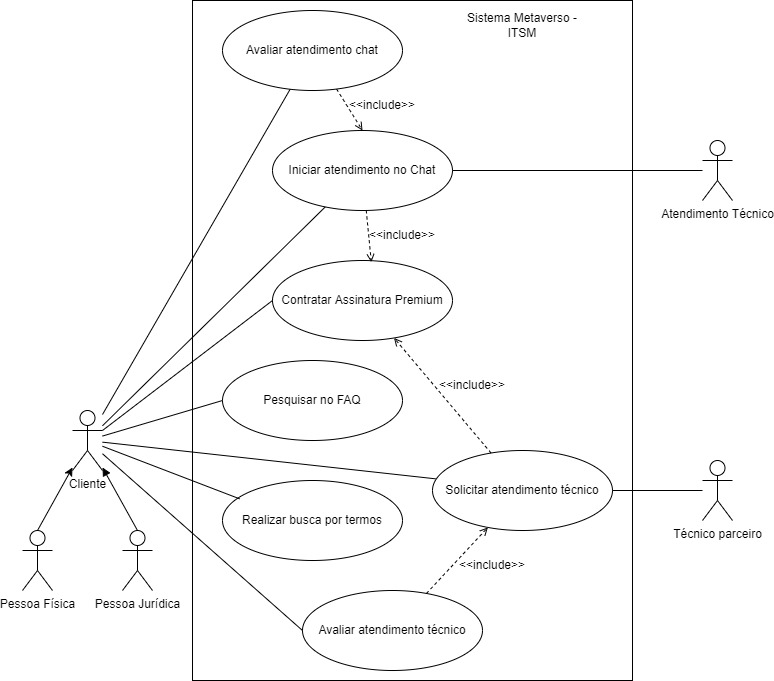
\includegraphics[width=15cm]{anexos/Casos de Uso.jpeg} % leia abaixo
\label{figura:casosdeuso}
\fonte{Os Autores}
\end{figure}

Os casos de uso orientam a equipe de desenvolvimento sobre o que a aplicação deverá atender. Conforme diagrama acima, vemos 3 atores principais e suas generalizações, além de suas atividades dentro da aplicação. Assim, podemos dividi-lo nos seguintes casos de uso:

\subsection{Caso de Uso: Contratar Assinatura Premium}
O cliente, que pode ser pessoa física ou jurídica, se torna um assinante Premium da aplicação, mediante pagamento mensal de um valor pré-determinado, de acordo com o plano contratado. Alguns dos próximos casos de uso estão vinculados ao usuário ter a assinatura ativa para conseguir utilizar.

\subsection{Caso de Uso: Pesquisar no FAQ}
O cliente navega dentro do FAQ, visualizando categorias que levem-o até o problema que o mesmo tenha e disponibilize uma solução.

\subsection{Caso de Uso: Realizar busca por termos}
O cliente poderá, após a pesquisa no FAQ sem sucesso, realizar uma busca dentro da própria aplicação através de poucas palavras que poderá indicar links de outros sites e fóruns potencialmente úteis para solucionar seu problema.

\subsection{Caso de Uso: Iniciar atendimento no Chat}
O cliente poderá a qualquer momento, desde que seja um assinante Premium ativo, iniciar um atendimento técnico via chat, onde terá auxílio para resolver os problemas técnicos de seu dispositivo.

\subsection{Caso de Uso: Avaliar atendimento Chat}
O cliente que tiver passado por um Atendimento via chat, conforme mencionado no caso anterior, poderá avaliar o atendimento, contribuindo para a melhoria da aplicação e parceiros.

\subsection{Caso de Uso: Solicitar atendimento técnico}
O cliente pode solicitar um atendimento técnico, que poderá ser multicanal(telefone, mensagens, remota ou presencial) de um técnico parceiro. A ferramenta listará os técnicos da região disponíveis para atender o chamado de acordo com sua especialidade, onde o cliente pode escolher o técnico ou deixar em aberto para que os técnicos possam aplicar para atender o atendimento.

\subsection{Caso de Uso: Avaliar o atendimento técnico}
O cliente que tiver solicitado atendimento técnico avalia o mesmo, contribuindo para a relevância do Técnico parceiro dentro da ferramenta e para possíveis melhorias dentro da plataforma.

\section{Regras de negócio}
\section{Requisitos Funcionais}
\section{Requisitos Não Funcionais}
\section{MER e DER}

%\section{Justificativa}

%\section{Estrutura do Estudo}

%\lipsum[3-5]
%Teste de citação para gerar referências no modelo.. \citeauthor{SCRUMGUIDE:2013}

% ----------------------------------------------------------
% Referências bibliográficas
% ----------------------------------------------------------
\bibliography{referencias,exemplos/abntex2-doc-abnt-6023}

\end{document}